\documentclass[conference]{IEEEtran}
\IEEEoverridecommandlockouts
% The preceding line is only needed to identify funding in the first footnote. If that is unneeded, please comment it out.
\usepackage{cite}
\usepackage{amsmath,amssymb,amsfonts}
\usepackage{algorithmic}
\usepackage{graphicx}
\usepackage{textcomp}
\usepackage{xcolor}
\usepackage{anyfontsize}

\def\BibTeX{{\rm B\kern-.05em{\sc i\kern-.025em b}\kern-.08em
    T\kern-.1667em\lower.7ex\hbox{E}\kern-.125emX}}
\begin{document}

\title{Machine Learning Based Human Attention Recognition From Brain-EEG Signals}



\author{\IEEEauthorblockN{Reshad Hassan\textsuperscript{\authorrefmark{1}}, Sakib Hasan\textsuperscript{\authorrefmark{2}},
Md. Jubaer Hasan\textsuperscript{\authorrefmark{3}}, 
Md. Rafat Jamader\textsuperscript{\authorrefmark{4}},
David Eisenberg\textsuperscript{\authorrefmark{5}} and
Tanmoy\thanks{*Corresponding Author : tsr@uap-bd.edu} Pias\footnotemark\textsuperscript{\authorrefmark{*6}}}

\IEEEauthorblockA{Department of CSE, University of Asia Pacific, Bangladesh \& Virginia Tech, USA\\}

\IEEEauthorblockA{ \{17201069\textsuperscript{\authorrefmark{1}}, sakib.hasan\textsuperscript{\authorrefmark{2}}, 17201070\textsuperscript{\authorrefmark{3}} , 17201076\textsuperscript{\authorrefmark{4}}, tsr\textsuperscript{\authorrefmark{*6}}\} @uap-bd.edu, davide77@vt.edu\textsuperscript{\authorrefmark{5}}}
}


\maketitle

\begin{abstract}
Emotion recognition has always been a very popular field of research. Recently, EEG brain waves are being used to recognize the emotional states of a person. Attention level also plays an
important role in human life but still demands more investigation. This paper proposes a cost-effective, single-channel, time-frequency scalp-EEG signals-based noble human attention level recognition system using
advanced machine learning algorithms. In this study, the Bitalino EEG sensor board has been used to record EEG signals from 30 human subjects in different attention states. Initially, the attention level was classified into three categories, which are focused, neutral and distracted. The data was taken while the subjects were watching interesting videos and boring lectures, doing simple and interesting math problems, and solving interesting and hard puzzles. At first, these EEG signals are pre-processed to remove noise such as muscle movement. Statistical coefficients (i.e. mean, standard deviation, skewness, kurtosis, and entropy) and statistical wavelet transform are used to extract meaningful features from the EEG signal. We mainly used two Multi-scale Wavelet Packet Statistics (WPS) and Multi-scale Wavelet Packet Energy Statistics (WPES) to generate the feature vector. This feature vector was used to train the complex hybrid model with CNN and LSTM. This proposed method achieved almost 89\% accuracy while determining the attention level of a subject.



\end{abstract}

\begin{IEEEkeywords}
EEG(Electroencephalography), Brainwave, Wavelet Decomposition, Deep Learning etc.  
\end{IEEEkeywords}

\section{Introduction}
The study of the brain has always fascinated mankind. Whether in the medical sciences, psychology, or computer science, brain research promises hope for a better understanding of ourselves and our society.  The study of brain signals has helped not only to detect brain tumors from an Electroencephalograph, but has even helped cure brain-related diseases like Alzheimer’s disease\cite{b5}, sleep disorders\cite{b1} or driver’s fatigue\cite{b9}.

Whatever the human body does affects the brain. Electrons flow across neurons, produce a variance in EEG signals. Researchers addressing these changes in Brain-EEG signals produced a variety of experiments \cite{b2, b4, b6, b10, b11}, where authors demonstrated how Machine Learning approaches can be used in emotional states classification. Albeit numerous experiments have taken place in detecting diseases or classifying human emotions, no one has specifically addressed Human Attention level recognition. 


So what is Human Attention Level?  Simply put, it refers to the different states of the human brain that occur while you are putting your brain to any task.  For instance, a student can be either attentive or inattentive during a lecture when the brain's functionality won't match.  In this paper, we have addressed Human Attention Level recognition using students as the focus of this sample. 

Though the majority of the data collections for these studies consist of students, attention level can also be studied in various other domains, including office employees, commercial drivers, pilots, etc. Our work has developed a novel Machine Learning and Deep Learning-based Human Attention Level recognition model using Brain-EEG, which can identify the attention level of any single human being at an instance.


\section{The Specifics of Electroencephalography}
\label{eeg}
\subsection{Composition of a raw EEG signal}
Electroencephalography(EEG) is an electro-physiological measurement technique used to record the electrical movement of the cerebrum. It is noninvasive, with the terminals set along the scalp, albeit obtrusive cathodes are now and again utilized, as in electro-corticography. EEG measures voltage vacillations coming about because of ionic current inside the neurons of the cerebrum.

A raw EEG signal(Fig. 4) consists of several frequency sub-bands: Gamma(\textgreater30Hz), Beta(13-30Hz), Alpha(8-12 Hz), Theta(4-8Hz), and Delta(\textless4Hz). But a raw EEG captured from any human interferes from a lot of Noises on account of unwanted Muscular movements or outside phenomena\cite{b14}. 

Previous research \cite{b3} has provided a clear picture of how raw EEG signals can be decomposed into sub-bands. In our present work, we used some advanced functions of Matlab2019a, based on this model in Fig.1


\begin{figure}[htbp]
\centerline{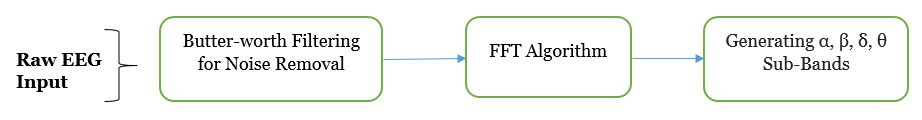
\includegraphics[scale=.4]{figures/Decomposing_wf.JPG}}
\caption{Workflow to decompose raw EEG}
\label{fig}
\end{figure}



\subsection{Machine Learning and Deep Learning studies on EEG}
Research regarding the ML and DL-based classification of different brain states, diseases, and emotional states has been undertaken for quite some time. A comparative analysis of different Machine Learning algorithms’ performances \cite{b1, b8} attempted to classify these EEG signals.  \textit{Bhardwaj et. al.} \cite{b9} presented us with a in depth analysis of different ML and DL-based algorithms while classifying EEG signals. In that paper, the authors compared SVM, KNN, DT, Autoencoder, and Ensemble.

In another study, \textit{Lin et. al.} \cite{b6} attempted to classify human emotions while subjects listened to music.  This approach was improved upon by \textit{Peng et. al.} \cite{b7}, when they used manifold regularized extreme learning machine using advanced algorithms like GELM, MRELM etc. over SVM.

The basics of EEG breakdown is previously described in simple terms \cite{b3}, whereas \textit{Kher et. al.} described how to capture raw EEG signals with wireless transmission \cite{b14}.  With time, we saw the uses of recent ML and DL algorithms for classifying EEG signals.  With advanced algorithms like LSTM-RNN, \textit{Jeevan et. al} \cite{b4} recognized different human emotions with higher accuracy.  \textit{Amin et. al.} \cite{b10} took on Pattern Recognition approaches to classify EEG signals.  Deep recurrent convolutional neural networks was subsequently used to classify EEG by \textit{Bashivan et. al} \cite{b11}, and likewise, \textit{Subasi et. al.} \cite{b13} used mixture of expert models with the same intention. 

Apart from these examples, EEG signal classification is used in detecting diseases including, but not limited to, Seizures, Alzheimer’s disease, Driver’s fatigue stages, Human sleeping stages, Brain Tumor, Strokes, and Dementia.

\section{Human Attention Recognition and Our Proposal}\label{hal}
No one can maintain 100\% attention at every moment while listening to an entire lecture.  At times, one adheres to his/her studies fully (\textbf{Attentive Mode}), sometimes that person will enter into an excited state (\textbf{Happy or Sad}), and sometimes s/he just does nothing (\textbf{Neutral Mode}).  

Although much work has been done on classifying human emotions and diseases, almost no work has targeted human attention levels. The changes
in human EEG signals during different attention levels for students have never been taken into consideration for study.  

In this paper, we devised a novel machine learning-based Human Attention recognition model using raw Brain-EEG signals. We built our own data-set for training and testing, and designed a complex hybrid
model using CNN \& LSTM.

\section{Data Collection and Setup}
\label{AA}

\subsection{Device used : Bitalino}
For data collection we used the "(R)evolution Plugged Kit BT" from \textit{Bitalino Inc.(\textit{https://bitalino.com/en/})}. This device features ability to capture EEG, ECG, EMG, EDA signals and also comes with a software which stores the real-time data in the host workstation in \textit{text} or \textit{edf} format.

\subsection{Target Audience and Our Data}
There were 20 participants, for which the EEG signal was recorded twice from each participant. Therefore, we have 40 unique instances of EEG Brain signals. Each instance of EEG was eight minutes (480 seconds) long. The signals that we have collected were from students attending the University of Asia Pacific, Bangladesh, all aged between 21 to 25 years.
  
\begin{figure}[htbp]
\centerline{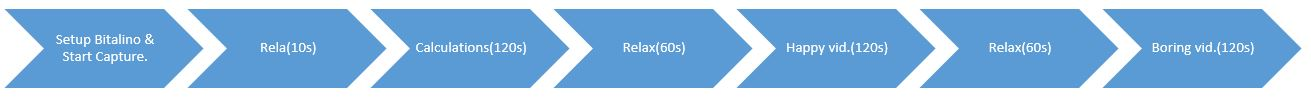
\includegraphics[scale=.35]{figures/Data_Capture.JPG}}
\caption{Data Capture process}
\label{fig}
\end{figure}
Fig. 2 provides our data collection procedure, and our methodology used to change the student’s attention states.

\section{Experimentation Setup}

\subsection{Data Pre-processing}\label{dp}
An important step in our data collection was manual labeling. At first, we observed how the signal looked in a neutral state.  We used three types of our data, which included Calculation, Happy, and Boring, as our attention levels. While a person was solving an interesting math problem, his EEG pattern changed abruptly.  However, this pattern does not persist throughout a whole session. That abruptly changed section of the pattern tells us the individual’s attention state from within the full raw EEG signal.

\begin{figure}[htbp]
\centerline{
\includegraphics[scale=.023]{figures/four_states.png}}
\caption{Neutral, Attentive, Happy, Boring States}
\label{fig}
\end{figure}

We recorded the start and end time of the attention period. The attention period and the attention level depended on both the nature of the task and the surrounding environment. After several tests, we found that the attention period normally lasted for 1-2 seconds.  Our goal was to classify a person’s states into four separate classes:  Neutral, Attentive, Happy, and Boring states. The attention state was manually segmented from the raw EEG signals. The sampling rate of the EEG signal was 1000Hz. The segment length is two seconds which consists of 2,000 data points. Every session (120 seconds) was segmented into 20 slots (consists of 2000 data points). Each of these slots represents an active attention zone.
 

\subsection{Feature Extraction}\label{fe}
The features can be classified into two types: time-domain and frequency-domain.  Time-domain features are statistical features, such as mean, variance, power, peak to peak difference, etc. Frequency-domain features are related to the decomposition of the raw signals into sub-signals.

In our experiment, the raw EEG was decomposed into sub-bands using a 1-D wavelet decomposition function in Matlab.  The signal was decomposed into eight levels, where each level represents different features. The detailed coefficient of levels 1 to 4 represents noise. Therefore, these four bands were removed from the analysis. The rest of the detail coefficients of wavelet decomposition levels 5 to 8 represent gamma, beta, alpha, and theta sub-signals. The approximation coefficient of level eight represents delta sub-bands. These sub-bands are very useful for EEG signal analysis (Fig. 4).

\begin{figure}[htbp]
\centerline{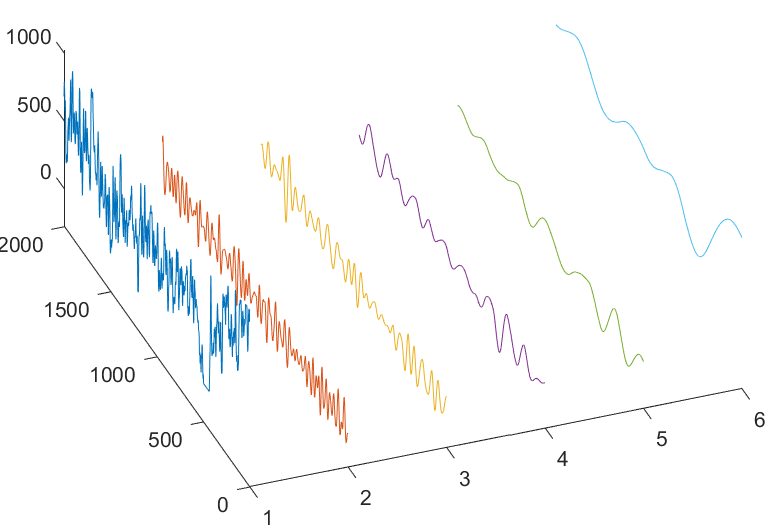
\includegraphics[height= 2.8cm, width = 6.5cm]{figures/data_pre.png}}
\caption{1-Raw, 2-gamma, 3-beta, 4-alpha, 5-theta, 6-delta. The length of the signal is 2000 and the z-axis represents the amplitude of the signals.}
\label{fig}
\end{figure}

Now we applied two functions on these sub-signals. One is \textbf{Welch’s Power Spectral Density Estimate(WPSDE)} and another function is \textbf{Spectrogram} using a short-time Fourier transform(STFT). The length of each sequence was 2 seconds where there were 2000 data points as the sampling rate was 1000Hz. Now, a number of statistical features were calculated considering a fixed window size of 100 milliseconds and the slide step size being 10 samples\footnote{1 sample= 1 milisecond}. Mean, Variance, Skewness, and Kurtosis were calculated from this signal using this sliding window configuration(Fig. 5). 

\begin{figure}[htbp]
\hbox{\hspace{-0.8em}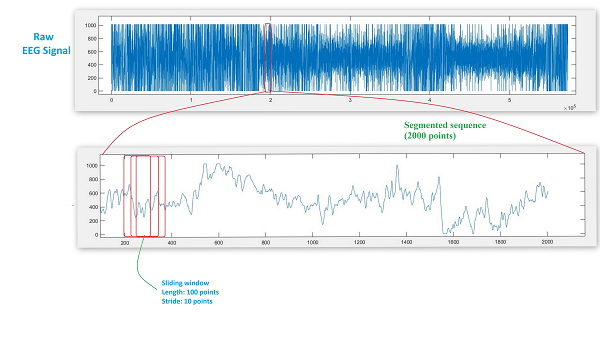
\includegraphics[scale=.08]{figures/Plot_example.png}}
\caption{Raw signal segmentation and sliding window for calculating statistical features}
\label{fig}
\end{figure}

\textit{Welch’s power spectral density estimation (WPSDE)} of all the sub-signals are taken as input features. Fig. 6. Demonstrates the WPSDE calculated from our dataset. The four statistical values are also taken as input features. The feature vector consists of 1 raw signal, 5 sub-signals, 24 statistical values (6 signals x 4 statistical formulae), with a Welch’s power spectral density estimation of six for each signal. In total, there were 48 values identified in in the feature vector.
 


\begin{figure}[htbp]
\centerline{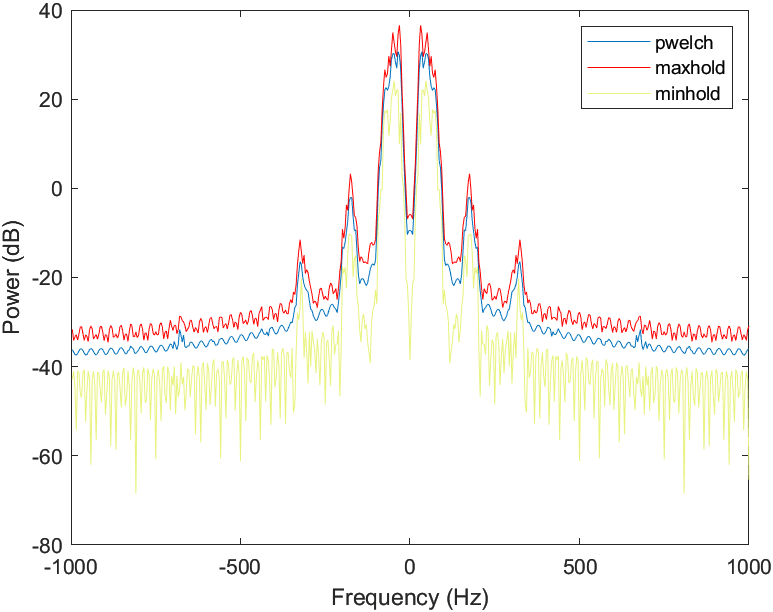
\includegraphics[width=8cm, height=4cm]{figures/welch.png}}
\caption{Welch’s Power Spectral Density Estimate}
\label{fig}
\end{figure}

\textit{Spectrogram of a signal} is the Power distribution in the time-frequency domain. The visual representation of the spectrogram is very important for signal analysis. Thus, the spectrogram function was applied to 6 signals. Among them, the spectrogram of raw, beta, and alpha signal was selected for analysis(Fig. 6). This selection was based on empirical reasoning and simulation of the deep learning model.

\begin{figure}[htbp]
\centerline{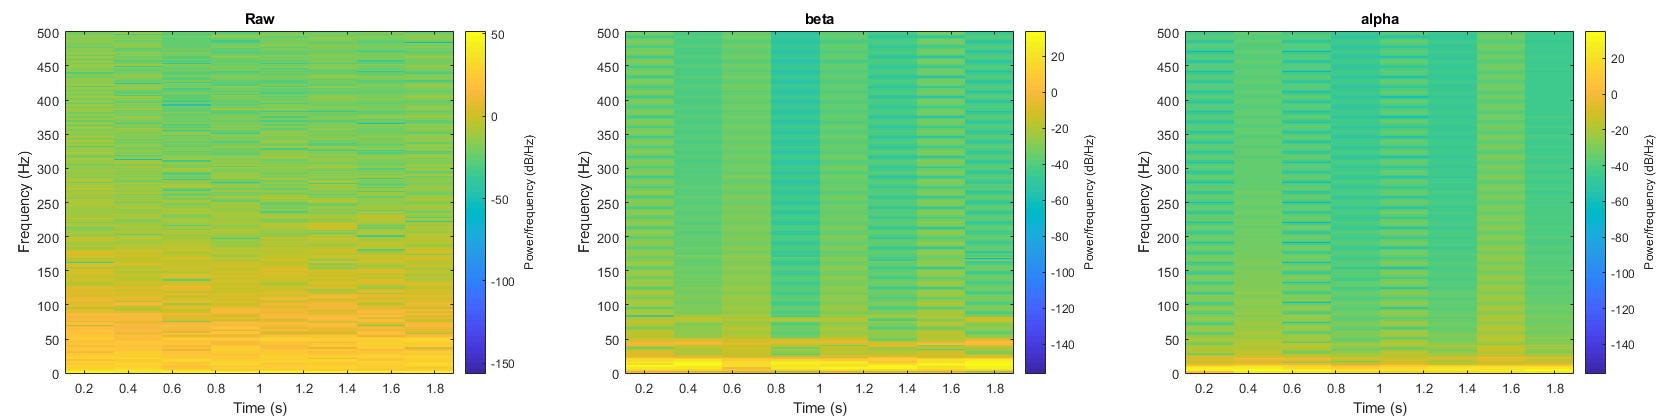
\includegraphics[scale=.15]{figures/spectrogram.jpg}}
\caption{Spectrogram of Raw, Beta and Alpha signal}
\label{fig}
\end{figure}

The digitally sampled data's power spectral density can be generalized to discrete time variables $x_n$. As above we can consider a finite window of $1\leq n\leq N$  with the signal sampled at discrete times $x_n$ = x(n$\Delta$t) for a total measurement period T = N$\Delta$t. Then a single estimate of the PSD can be obtained through summation rather than integration:

\begin{equation}
    \Tilde{S_{xx}}=\frac{(\Delta t)^2}{T}\mid {\sum_{n=1}^{N}x_ne^{-i\omega n \Delta t}} \mid ^2
\end{equation}

Here, $\omega$ is the window size for windowing, and N is the total no. of data points in the truncated signal \textbf{X}. x_n$ is the discrete time points from the truncated signal from signal transformed by STFT, and T being the total time period that signal is taken for. Side by side the Spectrogram of that same signal \textit{s(t)} is, S(t, \omega$)= \mid STFT(t, \omega$)\mid^2



\subsection{The Hybrid CNN-LSTM Model}
In our work, we built a Complex Hybrid model using \textit{CNN(Convolutional Neural Network)} and \textit{LSTM(Long-Short Term Memory)}. The LSTM is used for sequence classification. The data-set consists of a sequences and images. Each sequence is 2000 points long and has 48 features. Hence, the input dimension of LSTM is (40, 2000, 48) where 40 represents the instances of EEG. In paper \cite{b15, b16} a similar approach an artificial neural network was used for signal classification. 

\begin{figure}[htbp]
\centerline{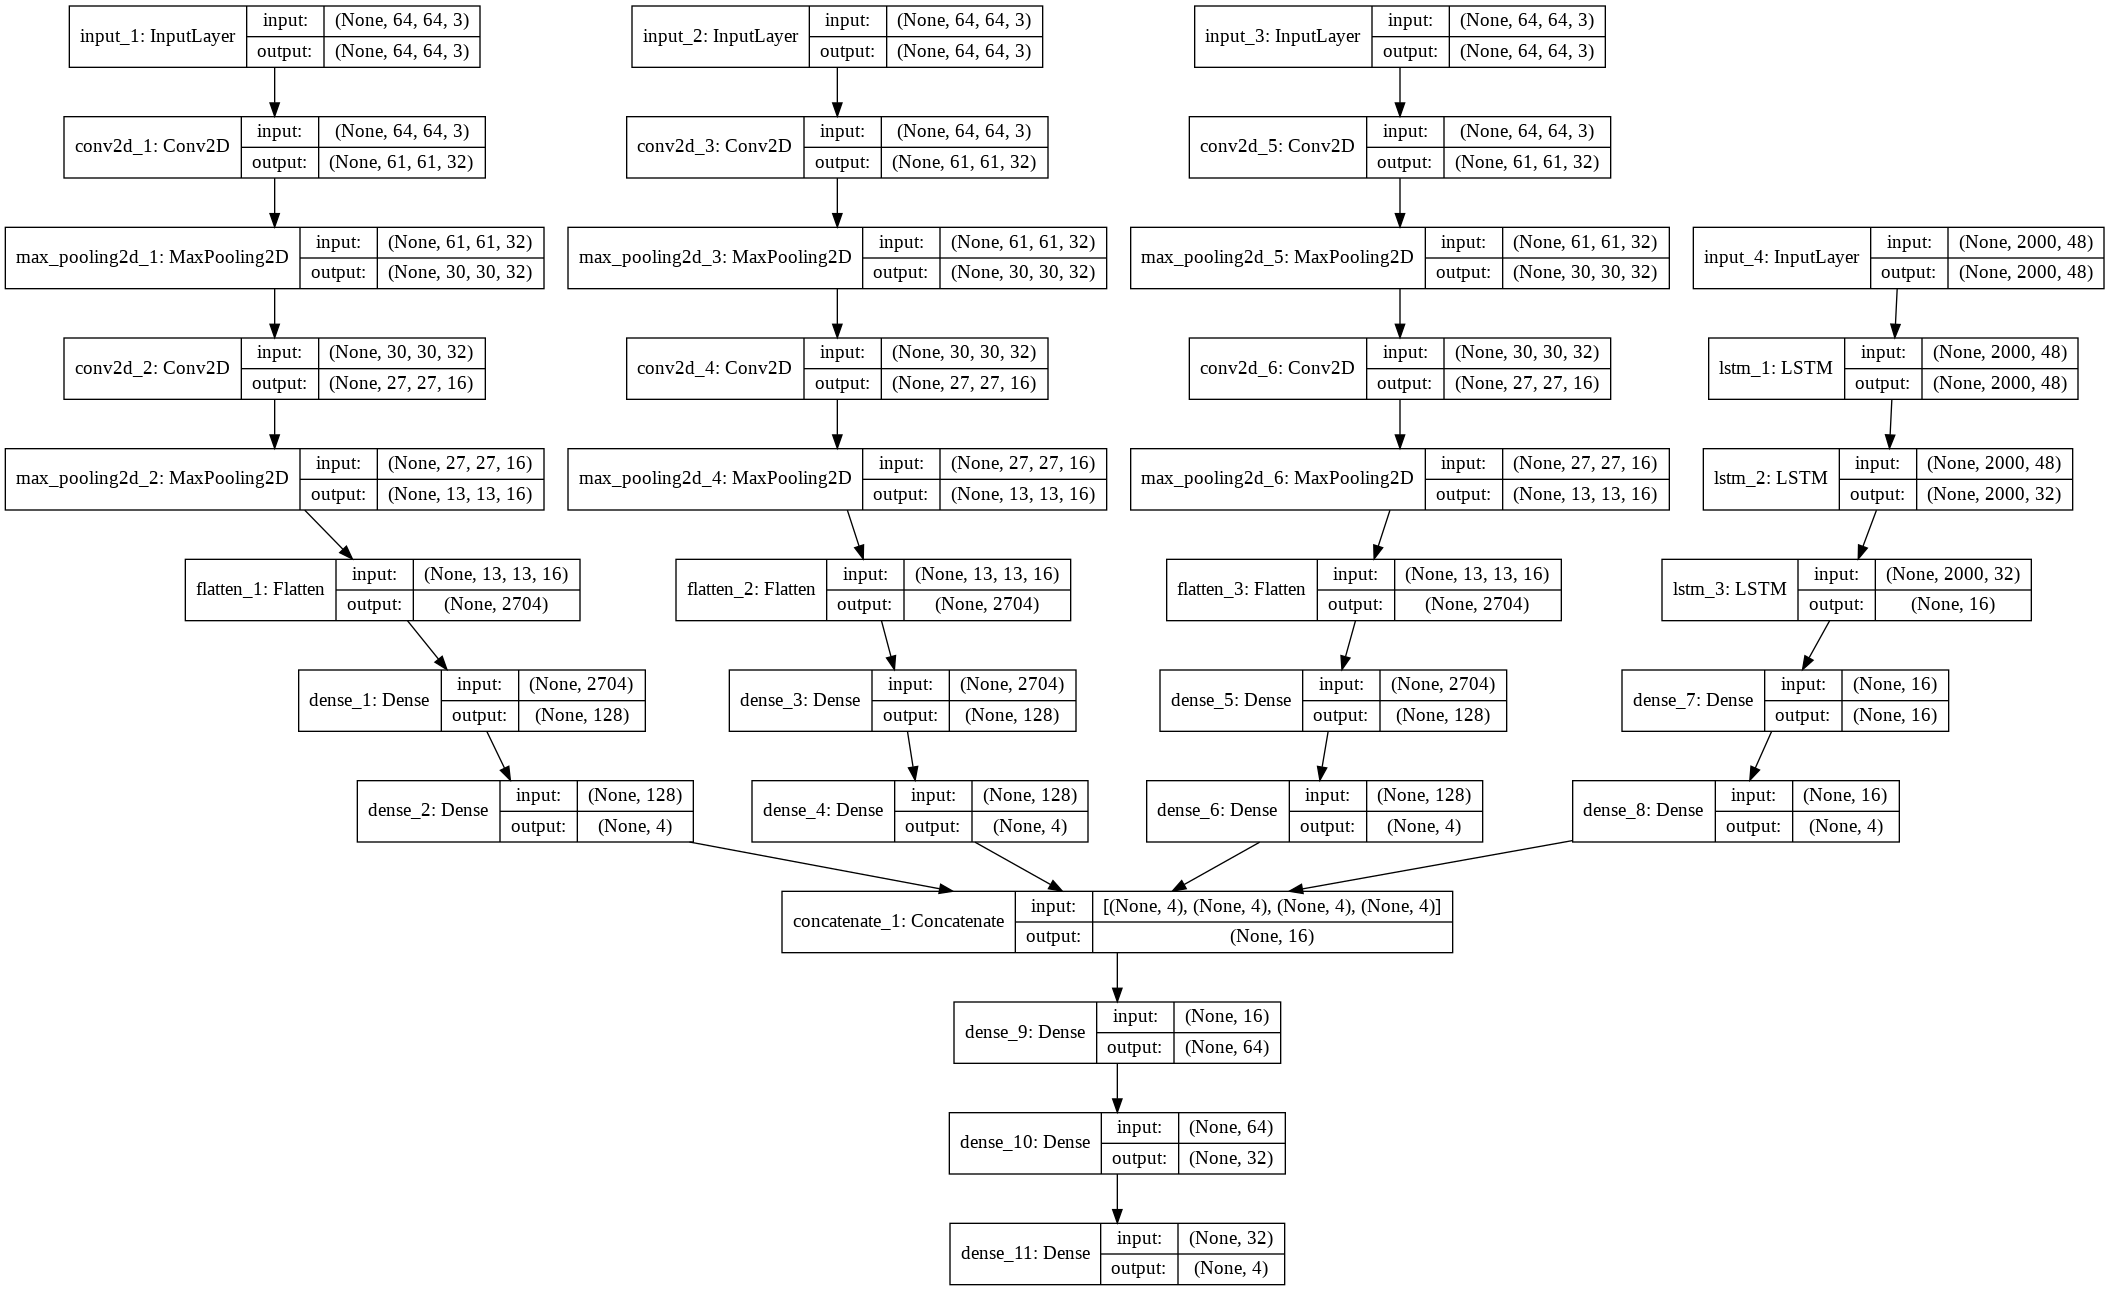
\includegraphics[width=8cm, height=8cm]{figures/cnn_lstm.png}}
\caption{Hybrid Deep Learning Model}
\label{fig}
\end{figure}

The visual data-set consists of a spectrogram of raw EEG, as well as beta and alpha signals. All of the spectrogram images were converted into 64x64x3 dimensions where 64x64 represents the height and width and 3 represents the RGB layers. Three CNN input layers take spectrograms of raw, beta, and alpha signals. In addition, one LSTM input layer takes the sequential input.  The output layer from each sub-model was concatenated into one layer followed by dense layers.

\section{Experiment Result Analysis}

The whole data pre-processing and feature extraction was done on \textit{Matlab 2019a}, whereas the model was trained and tested on a \textit{Kaggle} kernel.

The developed learning model acquired an astounding accuracy of 89\% which can differentiate among Neutral, Attentive, Happy or Sad. The model, during our calculation, takes about .0125 second for it's learning period. The deficiency in accuracy has occurred due to under saturation of data as our data-set is not adequate enough to train up the complex model we built. 

\section{Future Works}
With relation to this developed model, we will be focusing on two main future targets. First, we believe our data-set contained average numbers of data that need to be increased to a larger data-set. In this way, we aim to secure higher accuracy for our model with an increased number of features.  A community-based implementation of our model to create a Classroom Attention Level Recognition system would then be able to capture numerous EEG signals at once and process them for an ultimate result.


\section{Conclusion}
In the present study, a novel model using deep learning methods is devised for human attention states recognition.  Four states are defined for different levels of attention.  After filtering and the segmentation processes, spectral density and spectrogram analyses were implemented to retrieve features from the EEG recordings. The CNN-LSTM based model is used as a classifier, which after experimenting on our self-built data-set illustrated that a satisfactory and empirical execution can be reached through the proposed framework.


\section*{ACKNOWLEDGMENT}
This research is supported financially by the Institute for Energy, Environment, Research and Development(IEERD), University of Asia Pacific located in Dhaka, Bangladesh. Therefore, we would like to express our heartfelt gratitude to them for the financial support we received for the project.



\begin{thebibliography}{00}
\bibitem{b1} Aboalayon, Khald AI, Wafaa S. Almuhammadi, and Miad Faezipour. "A comparison of different machine learning algorithms using single channel EEG signal for classifying human sleep stages." In 2015 Long Island Systems, Applications and Technology, pp. 1-6. IEEE, 2015.

\bibitem{b2} Jalilifard, Amir, Ednaldo Brigante Pizzolato, and Md Kafiul Islam. "Emotion classification using single-channel scalp-EEG recording." In 2016 38th Annual International Conference of the IEEE Engineering in Medicine and Biology Society (EMBC), pp. 845-849. IEEE, 2016.

\bibitem{b3} C.Jaganathan, A.Amudhavalli, T.Janani, M. Dhanalakshmi, Nirmala Madian. “Automated algorithm for extracting α, β, δ, θ of a human EEG.” In 2015 International Journal of Science, Engineering and Technology Research (IJSETR) (Vol. 4, Issue 4)

\bibitem{b4} Jeevan, Reddy Koya, SP Venu Madhava Rao, Pothunoori Shiva Kumar, and Malyala Srivikas. "EEG-based emotion recognition using LSTM-RNN machine learning algorithm." In 2019 1st International Conference on Innovations in Information and Communication Technology (ICIICT), pp. 1-4. IEEE, 2019.

\bibitem{b5} Ieracitano, Cosimo, Nadia Mammone, Alessia Bramanti, Silvia Marino, Amir Hussain, and Francesco Carlo Morabito. "A Time-Frequency based Machine Learning System for Brain States Classification via EEG Signal Processing." In 2019 International Joint Conference on Neural Networks (IJCNN), pp. 1-8. IEEE, 2019.

\bibitem{b6} Lin, Yuan-Pin, Chi-Hong Wang, Tzyy-Ping Jung, Tien-Lin Wu, Shyh-Kang Jeng, Jeng-Ren Duann, and Jyh-Horng Chen. "EEG-based emotion recognition in music listening." IEEE Transactions on Biomedical Engineering 57, no. 7 (2010): 1798-1806.

\bibitem{b7} Peng, Yong, Jia-Yi Zhu, Wei-Long Zheng, and Bao-Liang Lu. "EEG-based emotion recognition with manifold regularized extreme learning machine." In 2014 36th Annual International Conference of the IEEE Engineering in Medicine and Biology Society, pp. 974-977. IEEE, 2014. 

\bibitem{b8} Dhivya, S., and A. Nithya. "A Review on Machine Learning Algorithm for EEG Signal Analysis." In 2018 Second International Conference on Electronics, Communication and Aerospace Technology (ICECA), pp. 54-57. IEEE, 2018.

\bibitem{b9} Bhardwaj, Rahul, Swathy Parameswaran, and Venkatesh Balasubramanian. "Performance Comparison of Machine Learning and Deep Learning While Classifying Driver’s Cognitive State." In 2018 IEEE 13th International Conference on Industrial and Information Systems (ICIIS), pp. 89-93. IEEE, 2018.

\bibitem{b10} Amin, Hafeez Ullah, Wajid Mumtaz, Ahmad Rauf Subhani, Mohamad Naufal Mohamad Saad, and Aamir Saeed Malik. "Classification of EEG signals based on pattern recognition approach." Frontiers in computational neuroscience 11 (2017): 103.

\bibitem{b11} Bashivan, Pouya, Irina Rish, Mohammed Yeasin, and Noel Codella. "Learning representations from EEG with deep recurrent-convolutional neural networks." arXiv preprint arXiv:1511.06448 (2015).

\bibitem{b12} Liao, Chung-Yen, and Rung-Ching Chen. "Using Eeg Brainwaves And Deep Learning Method For Learning Status Classification." In 2018 International Conference on Machine Learning and Cybernetics (ICMLC), vol. 2, pp. 527-532. IEEE, 2018.

\bibitem{b13} Subasi, Abdulhamit. "EEG signal classification using wavelet feature extraction and a mixture of expert model." Expert Systems with Applications 32, no. 4 (2007): 1084-1093.

\bibitem{b14} Kher, Rahul K., and Rathang U. Shah. "Wireless EEG Signal Acquisition and Device Control." In researchgate.com(2016)

\bibitem{b15} Pias, Tanmoy Sarkar, David Eisenberg, and Muhammad Aminul Islam. "Vehicle Recognition Via Sensor Data From Smart Devices." In 2019 IEEE Eurasia Conference on IOT, Communication and Engineering (ECICE), pp. 96-99. IEEE, 2019.

\bibitem{b16} Pias, Tanmoy Sarkar, Raihan Kabir, David Eisenberg, Nadeem Ahmed, and Md Rashedul Islam. "Gender Recognition by Monitoring Walking Patterns via Smartwatch Sensors." In 2019 IEEE Eurasia Conference on IOT, Communication and Engineering (ECICE), pp. 220-223. IEEE, 2019.

\end{thebibliography}


\end{document}
